\documentclass{article}

\usepackage[version=3]{mhchem}
\usepackage[greek,english]{babel}
\usepackage{booktabs}
\usepackage{gensymb}
\usepackage{graphicx}
\usepackage[hidelinks]{hyperref}
\usepackage{fixltx2e}
\usepackage{titlesec}
\usepackage[normalem]{ulem}
\usepackage{parskip}
\usepackage{multirow}
\usepackage{fancyvrb}
\usepackage{color}
\usepackage{float}
\usepackage[super]{nth}

\titleformat*{\section}{\Large\bfseries}
\titleformat*{\subsection}{\bfseries}

\hypersetup{
  colorlinks   = true,
  urlcolor     = blue,
  linkcolor    = black,
  citecolor    = black
}

\definecolor{grey}{gray}{0.75}

\newfloat{listing}{thp}{lop}
\floatname{listing}{Listing}

\setcounter{secnumdepth}{0}

\newcommand{\calpha}{C\textsubscript{\textgreek{a}}}
\newcommand{\ahelices}{\textgreek{a}-helices}
\newcommand{\bsheets}{\textgreek{b}-sheets}
\newcommand{\bbphi}{\ensuremath{\phi}}
\newcommand{\bbpsi}{\ensuremath{\psi}}
\newcommand{\bbomega}{\ensuremath{\omega}}
\newcommand{\module}[2]{\href{#2}{\texttt{#1}}}
\newcommand{\atomrec}{\texttt{ATOM} record}

\begin{document}

\title{Making Ramachandran Plots}
\author{2014 iPQB Bootcamp\\Summer Programming Project}
\date{}
\maketitle{}

\section{Introduction}

The purpose of this project is to help you learn Python by giving you 
challenging but relevant problem to practice on.  The project is to write a 
program that generates Ramachandran plots from PDB files.  Ramachandran plots 
show how backbone torsion angles are distributed in proteins.  Different 
features of proteins (namely \ahelices{} and \bsheets{}) occupy distinct 
regions in these plots.  For this reason, Ramachandran plots are commonly used 
both to validate experimental structures and to predict computational 
structures.

Hopefully, this project will require you to exercise three skills that are 
essential for scientific programming:

\begin{enumerate}
 \item Reading in data from a file.
 \item Manipulating that data numerically.
 \item Plotting your results.
\end{enumerate}

If you have any questions about programming or this project, send me an email 
at \href{mailto:kale.kundert@ucsf.edu}{kale.kundert@ucsf.edu}.

\section{What is a Ramachandran Plot?}

I'll explain exactly what a Ramachandran plot is below, but I'll begin by 
introducing some basic terminology.  This is necessarily a brief introduction, 
so feel free to email me for clarification if you get lost.  First of all, 
proteins are composed of amino acid residues.  Figure \ref{fig:three-residues} 
shows three residues from a larger protein.  A distinction is made between the 
backbone (blue) and the sidechains (red).  Every residue in the protein is 
connected through the backbone, which has a very regular pattern of atoms: 
\ce{N - C_{\textgreek{a}} - C - N - C_{\textgreek{a}} - C - \ldots} where the 
carbon that supports the sidechain is called \calpha{} to distinguish it from 
the one that doesn't.

\begin{figure}
 \centering
 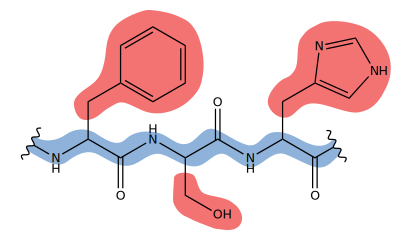
\includegraphics[width=0.8\textwidth]{three-residues}
 \caption{Three residues with the backbone and sidechains highlighted.}
 \label{fig:three-residues}
\end{figure}

Torsion angles are a convenient way to describe the geometry of the backbone.  
A torsion angle can be intuitively described the amount of twist around a bond.  
To be more precise, consider four consecutive backbone atoms.  You always need 
four atoms to define a torsion angle.  Use the first three atoms to construct 
one plane and the last three atoms to construct another.  The angle between 
those two planes is the torsion angle, or the twist around the bond connecting 
the second and third atoms.  These angles are convenient way to describe 
geometry because they don't depend on the orientation of whole protein in 
Cartesian space.

For each residue in a protein, three backbone torsions are defined:

\begin{table}[h]
\centering
\begin{tabular}{ll}
\toprule
Torsion      & Backbone Atoms                                               \\
\midrule
$\omega{}_i$ & \ce{
C^{$i$-1}_{\textgreek{a}} - C^{$i$-1} - N^{$i$} - C^{$i$}_{\textgreek{a}}}  \\
$\phi{}_i$ & \ce{
C^{$i$-1} - N^{$i$} - C^{$i$}_{\textgreek{a}} - C^{$i$}}                    \\
$\psi{}_i$ & \ce{
N^{$i$} - C^{$i$}_{\textgreek{a}} - C^{$i$} - N^{$i+1$}}                    \\
\bottomrule
\end{tabular}
\caption{Backbone torsion angles.}
\label{tab:backbone-torsions}
\end{table}

A Ramachandran plot is a scatter plot showing the \bbphi{} and \bbpsi{} angles 
for each residue.  The \bbphi{} angles are plotted along the x-axis and the 
\bbpsi{} angles are plotted along the y-axis.  Each point is the $\phi_i, 
\psi_i$ pair for one residue.  The \bbomega{} angles are left out because they 
never deviate much from 180\degree.  

Figure \ref{fig:example-plot} shows the Ramachandran plot for PDB ID: 1AXC, 
which is one of the structures you'll use for this project.  Note that there 
are two distinct clusters of points.  These represent two specific backbone 
conformations that are common in folded proteins: \ahelices{} (lower cluster) 
and \bsheets{} (upper cluster).  The ability to easily identify which residues 
are contributing to well-known, stable structural motifs is what makes 
Ramachandran plots useful for structural validation and prediction. 

\begin{figure}
 \centering
 \includegraphics[width=0.57\textwidth]{example-plot}
 \caption{Ramachardran plot for PDB ID: 1AXC}
 \label{fig:example-plot}
\end{figure}

\section{What Do You Need to Do?}

Your task is to create a program written in Python that takes a PDB file 
(specified on the command line) as input and produces a Ramachandran plot as 
output.  This is meant to be a challenging task for someone new to Python, so 
before starting you should work through an online tutorial.  There are lots of 
tutorials out there geared towards all different skill levels, but my favorite 
is \href{http://learnpythonthehardway.org/book}{Learn Python the Hard Way}.  
Once you get started, use the paragraphs below to guide how you write your  
program.  Some example inputs are also available for you to download from the 
\href{https://sites.google.com/site/ipqbbootcamp2014/programming}{bootcamp 
website}.

\subsection{Reading PDB Files}

PDB files contain information about the 3D structure of protein.  PDB stands 
for Protein Data Bank, which is online database of protein structures.  These  
files are regular text files (so you can view them using the same program you 
edit Python code with) where each line contains different information about the 
structure.  The lines containing the information relevant to this project all 
begin with the keyword \texttt{ATOM}.  

\begin{listing}[h]
\centering
\begin{BVerbatim}[fontsize=\footnotesize,commandchars=\\\{\}]
\textcolor{grey}{         1         2         3         4         5         6         7         8}
\textcolor{grey}{12345678901234567890123456789012345678901234567890123456789012345678901234567890}
ATOM   2305  CA  ILE A 255      35.578   9.357   5.792  1.00 43.22           C  
\end{BVerbatim}
\caption{An example \atomrec{}.}
\label{list:pdb-example}
\end{listing}

Listing \ref{list:pdb-example} shows an example \atomrec{}.  (The gray numbers 
aren't part of the record; they're just numbering the columns.)  Each 
\atomrec{} identifies a particular atom and specifies it's coordinates.  
Different pieces of information about the atom are always given at a fixed 
offset from the beginning of the line.  For example, the \nth{13} - \nth{16} 
characters of our example (\texttt{CA}) specify that the atom in question is a 
\calpha{}.  The \nth{18} - \nth{20} characters (\texttt{ILE}) specify that the 
atom is part of an isoleucine residue.
Table \ref{tab:pdb-atom-record} describes all of the \atomrec{} fields that are 
relevant to this project.  The complete 
\href{http://www.wwpdb.org/documentation/format33/v3.3.html}{PDB file format} 
is also available if you want more information.

\begin{table}[h]
\centering
\begin{tabular}{r@{ - }rcll}
\toprule
\multicolumn{3}{l}{Columns} & Example         & Description                         \\
\midrule
 1 &  6 & & \texttt{ATOM}   & Fixed string identifying each line. \\
 7 & 11 & & \texttt{7507}   & Atom serial number.                 \\
13 & 16 & & \texttt{CA}     & Atom name.                          \\
18 & 20 & & \texttt{ILE}    & Residue name.                       \\
23 & 26 & & \texttt{255}    & Residue sequence number.            \\
31 & 38 & & \texttt{35.578} & X coordinate of atom.               \\
39 & 46 & & \texttt{9.357}  & Y coordinate of atom.               \\
47 & 54 & & \texttt{5.792}  & Z coordinate of atom.               \\
\bottomrule
\end{tabular}
\caption{Description of the fields in an \texttt{ATOM} record.}
\label{tab:pdb-atom-record}
\end{table}

Learning how to break big problems into smaller problems is an important part 
of programming (and many other things).  When starting this project, don't try 
to write the whole thing at once.  Instead, take smaller steps.  Perhaps start 
by printing out all the lines in a PDB file.  Once that works, then try 
printing out only lines that correspond to backbone atoms.  Then try printing 
out only the Cartesian coordinates for those lines.  Once you have all that 
working, then start thinking about how to calculate torsion angles.

\subsection{Using Command Line Arguments}

Your program should accept the name of a PDB file as a command line argument.  
This will allow you to easily generate Ramachandran plots for different 
structures without having to change your script itself.  There are several ways 
to use command line arguments from python scripts.  If you're feeling 
overwhelmed and just want anything that works, look into 
\module{sys.argv}{http://learnpythonthehardway.org/book/ex13.html}.  If you're 
feeling more comfortable and want to learn how command line arguments are 
parsed in most modern python programs, look into 
\module{argparse}{https://docs.python.org/2.7/howto/argparse.html}.  And if you 
want to try an \texttt{argparse} alternative that beautifully marries parsing 
and documentation, look into \module{docopt}{https://github.com/docopt/docopt}.

\subsection{Calculating Torsion Angles}

Once you've read in Cartesian coordinates for all the backbone atoms, you'll 
need to calculate torsion angles.  This is not a trivial conversion, but you 
can find the algorithm 
\href{http://math.stackexchange.com/questions/47059/how-do-i-calculate-a-dihedral-angle-given-cartesian-coordinates}{here}.  

This algorithm involves a healthy dose of vector arithmetic.  Since python 
doesn't have built-in support for vector arithmetic, so you'll have to write 
write some vector arithmetic code yourself.  A vector is really nothing more 
than a set of three coordinates.  Use tuples to store these coordinates.  Then 
write and test functions to perform the following tasks:

\begin{enumerate}
 \item Add two vectors.
 \item Subtract two vectors.
 \item Normalize a vector.
 \item Calculate a dot product.
 \item Calculate a cross product.
\end{enumerate}

For example, your function that adds vectors would take two tuples as arguments 
and return their sum as a single tuple.  This is a good place to practice 
writing your own functions.  New programmers tend to copy-and-paste code in 
places where they should write functions.  Avoid that tendency here!

If you are feeling comfortable with functions and you want to learn more about 
object-oriented programming, try writing a vector class.  Classes are useful 
when you want to associate a particular set of data with a particular set of 
functions (usually called methods in this context).  Vectors make an ideal 
class, because the coordinates are clearly the data and the arithmetic helpers 
are clearly the methods.

If you are feeling comfortable with functions and classes, try performing these 
calculations using the 
\module{numpy}{http://wiki.scipy.org/Tentative_NumPy_Tutorial} vector math 
library.  This is a very important library for scientific programmers, because 
it makes it easy to work with large arrays of data.  It also makes Python feel 
more like Matlab in some ways, which might be appealing to those with a Matlab 
background.  Once you get past the learning curve, you'll find that 
\texttt{numpy} makes this calculation much easier.

\subsection{Making Plots}

Use \module{matplotlib}{http://matplotlib.org/users/pyplot_tutorial.html} to 
generate your Ramachandran plot.  The documentation for \texttt{matplotlib} is 
unfortunately pretty hard to understand, but the tutorial linked above isn't 
bad.  If you get stuck, feel free to send me an email.

\section{Future Directions}

If you found this project to be helpful, I've outlined several ways you can 
expand it to continue improving your ability as a scientific programmer.

\subsection{Make a residue-specific plot}

Glycine and proline have very distinctive Ramachandran plots.  Modify your 
program to either show just glycines, just prolines, or everything except 
glycine and proline.  There won't be enough glycines or prolines in a single 
structure to really show what these plots look like, so try combining this with 
the challenge below to fill in your plots.  Also, you might find it interesting 
to ponder why glycine and proline have distinctive plots if you don't already 
know.

\subsection{Make a combined plot for 10,000 structures}

Working with lots of data is an important skill for scientific programmers.  
Toward that end, I uploaded a subset of the CATH database comprising 11,926 PDB 
files to the website.  Download this data and modify your program to create a 
single Ramachandran plot for all of it.  Experiment with ways to speed up your 
program and to clearly present so many data points.

\subsection{Automatically download PDB files}

One of the nice things about Python is that it's not just for scientific 
programming, so there are libraries for doing things like downloading data from 
the web.  The PDB in particular makes it very easy to automatically download 
structures.  Modify your program to accept a PDB ID rather than an actual file, 
then download that structure from the PDB and use it to generate the plot.
The \module{requests}{http://docs.python-requests.org} library is a good place 
to start.

\end{document}
